\documentclass[12pt, a4paper]{article}
\usepackage[utf8]{inputenc}
\usepackage{graphicx}
\usepackage{geometry}
\usepackage{amsmath}
\usepackage{hyperref}
\usepackage{float}
\usepackage{booktabs}
\usepackage{siunitx}
\usepackage{grffile} % for spaces in file names

\geometry{margin=1in}

\title{\textbf{Scanning Tunneling Microscope}}
\author{Yamulapalli Nandu Navadeep \\ Roll Number: IMS24267}
\date{Date of the experiment: 02 September 2026 \\ Date of Submission: \today}

\begin{document}

\maketitle

\section{Name of the Experiment}
Scanning Tunneling Microscope (STM)

\section{Aim of the Experiment}
To understand the working principle of a Scanning Tunneling Microscope (STM), to operate the instrument using a sharp metal tip, and to obtain and analyze the topographical images of a gold-plated flat surface to study its nanoscale surface features.

\section{Theory}
The Scanning Tunneling Microscope (STM) is an instrument that allows us to visualize surfaces at the atomic level. Its operation is based on the quantum mechanical phenomenon of quantum tunneling. According to classical mechanics, a particle cannot overcome a potential barrier if its kinetic energy is lower than the potential energy of the barrier. However, in quantum mechanics, an electron has a non-zero probability of `tunneling' through the barrier.

In an STM, a sharp, tiny conducting needle (the tip) is brought very close (less than a nanometer) to a conductive sample surface. When a small bias voltage $V$ is applied between the tip and the sample, electrons can tunnel through the vacuum gap, creating a measurable tunneling current $I$. This current is highly sensitive to the distance $d$ between the tip and the sample, governed approximately by the relationship:
\begin{equation}
I \propto V \exp(-2 \kappa d)
\end{equation}
where $\kappa$ is a decay constant dependent on the work functions of the tip and the sample. Because of the exponential dependence, a small change in the distance $d$ results in a very large change in the tunneling current. This provides the STM with extraordinary vertical resolution.

The STM can operate in two primary modes:
\begin{itemize}
    \item \textbf{Constant Current Mode:} A feedback loop adjusts the tip's vertical position ($z$-axis) to maintain a constant tunneling current while scanning in the $x$ and $y$ directions. The recorded $z$-positions form the topographical map of the surface.
    \item \textbf{Constant Height Mode:} The tip scans across the surface at a fixed height, and the variations in tunneling current are recorded to form the image.
\end{itemize}
In this experiment, a piezo-electric scanner is used to accurately control the tip's position in three dimensions, allowing the mapping of the surface topography of a gold-plated sample.

\section{Procedure}
\begin{enumerate}
    \item \textbf{Sample and Tip Preparation:} A sharp STM tip was carefully inserted into the circular tip holder of the STM scanning head.
    \item A gold-plated flat plate was attached to the sample holder, which is a cylindrical block containing a magnet, and placed carefully into the STM apparatus.
    \item \textbf{Coarse Approach:} The STM head was placed over the sample, and the coarse approach mechanism was activated to bring the tip within a fraction of a millimeter of the sample surface using the motorized control, observing through a magnifying glass to avoid crashing the tip.
    \item \textbf{Fine Approach:} Using the control software on the computer, the automatic fine approach was initiated. The system slowly advanced the tip while monitoring the current until the setpoint tunneling current was established.
    \item \textbf{Scanning:} The software parameters were set, including the bias voltage, setpoint current, and scan area (e.g., $200\,\text{nm} \times 200\,\text{nm}$).
    \item The scan was started in constant current mode. Forward and backward scans for topographical (Z-axis) and tunneling current were recorded.
    \item The generated images were optimized by adjusting the integral and proportional gains of the feedback loop to minimize noise.
    \item \textbf{Analysis:} Line fits and mean fits were extracted across the scanned images to analyze the surface variations.

\end{enumerate}

\section{Tabular Column}
\begin{table}[H]
    \centering
    \caption{Typical Experimental Parameters for STM Scans}
    \begin{tabular}{@{}lc@{}}
        \toprule
        \textbf{Parameter} & \textbf{Value} \\
        \midrule
        Scan Area & $200\,\text{nm} \times 200\,\text{nm}$ \\
        Operating Mode & Constant Current \\
        \bottomrule
    \end{tabular}
\end{table}

\section{Calculations}
From the obtained line profile data in the software, the step heights and structural periodicity were calculated. For the topographical scan, the vertical height profile $z(x,y)$ reveals surface step structures. 

The vertical variation can be approximated by measuring the height difference $\Delta z$ between adjacent terraces on the line-fit graphs. 
\begin{equation}
\Delta z = |z_{\text{peak}} - z_{\text{valley}}|
\end{equation}
By averaging multiple steps along the cross-sectional line profile in the `Z-Axis - Scan forward' plot, one can determine the average size of the granules or height variation on the gold-plated surface.

\section{Results}
The scanning tunneling microscope successfully resolved the surface topography of the samples. 
\begin{itemize}
    \item The topographical scans of the gold-plated flat plate (shown in the Z-axis forward scans) indicate the presence of granular structures and distinct terraces typical of deposited gold films.
    \item The corresponding tip current images confirmed the stability of the scan, showing variations primarily around the step edges where the feedback loop is momentarily challenged by rapid height changes.
    \item The height profiles extracted across the surface showed a peak-to-valley roughness that characterizes the crystalline nature of the gold plating.
\end{itemize}

\section{Observation: }

\begin{figure}[H]
    \centering
    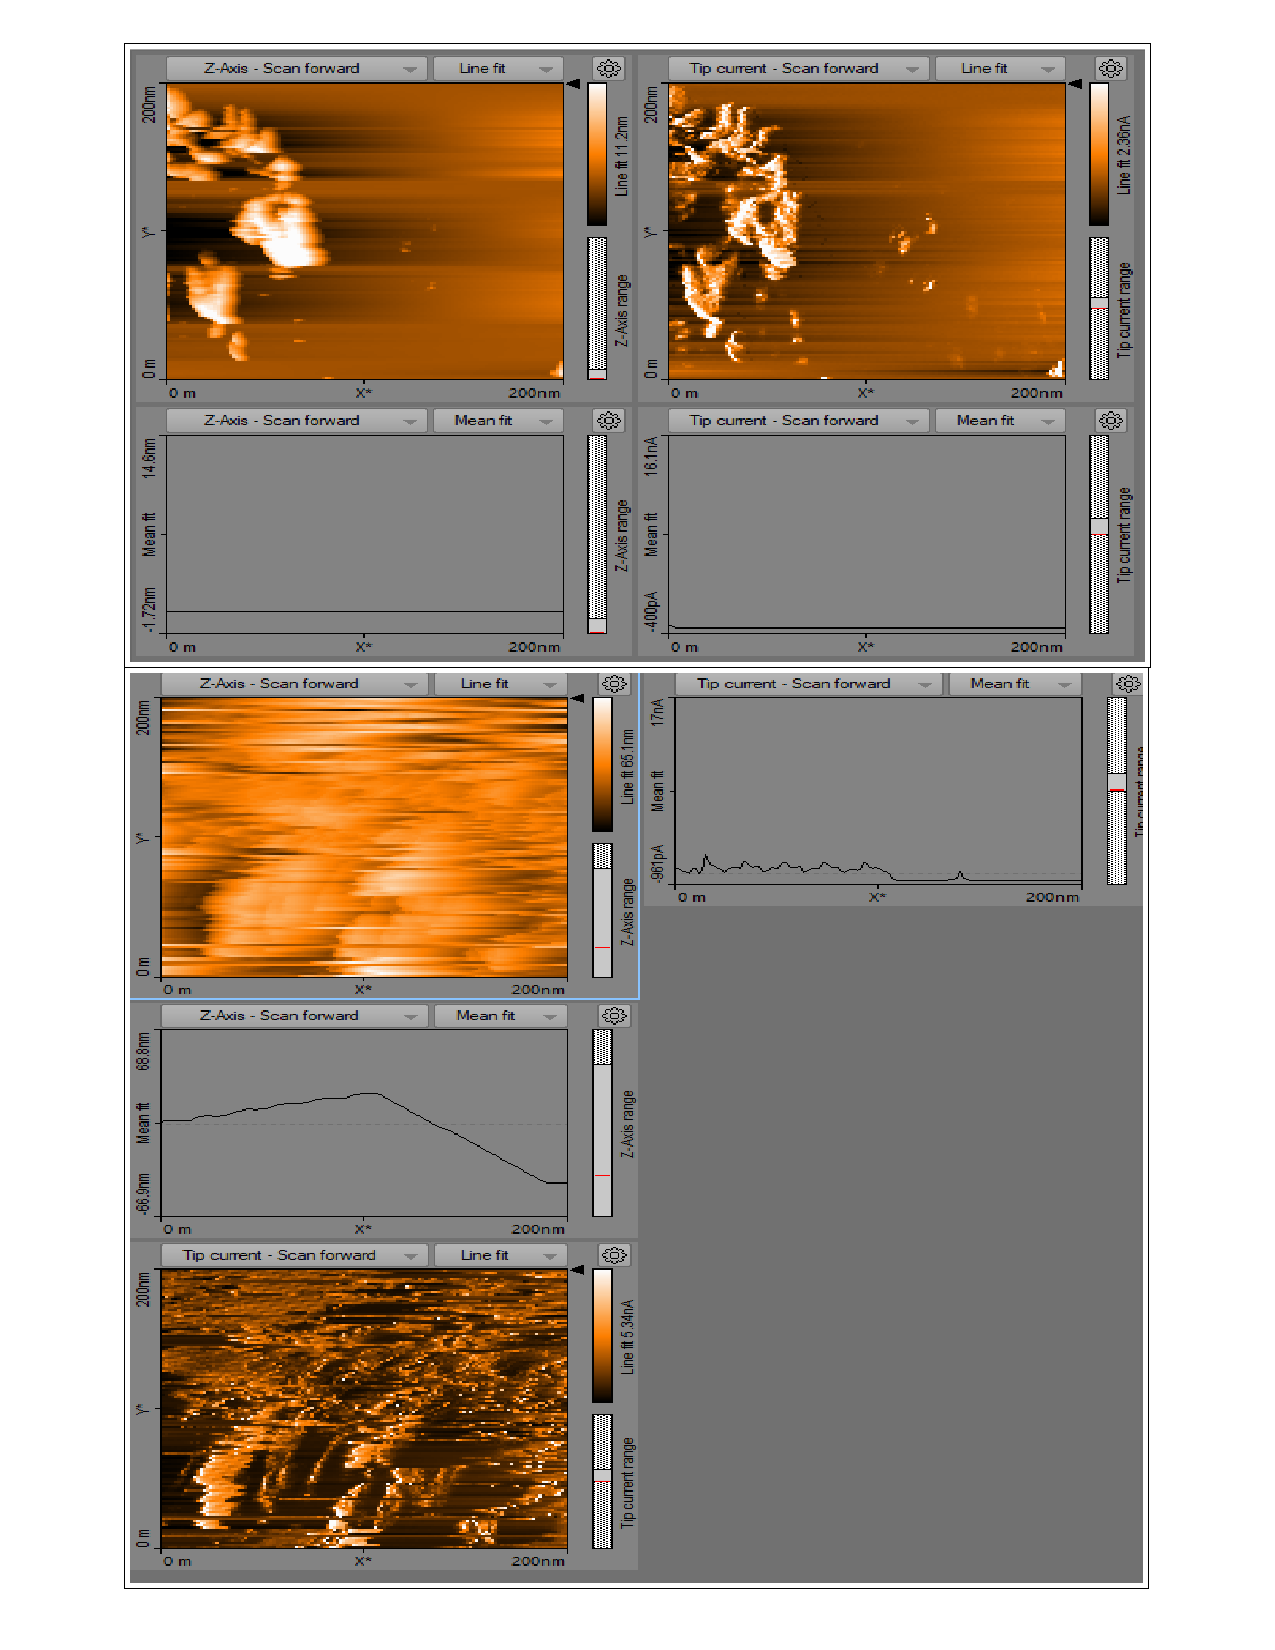
\includegraphics[width=0.9\textwidth]{print.pdf}
    \caption{STM scans of the sample, showing the Topography (Z-Axis) and Tip current variations for forward scans. The panels include line fits and cross-sectional height profiles over a $200\,\text{nm}$ region.}
    \label{fig:print}
\end{figure}

\begin{figure}[H]
    \centering
    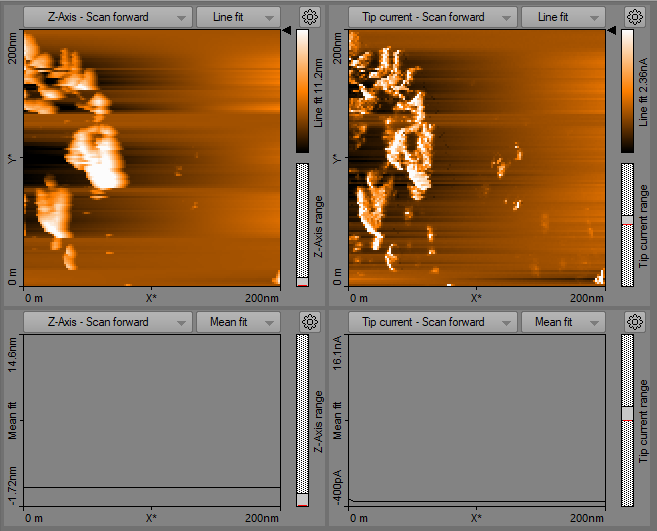
\includegraphics[width=0.7\textwidth]{1000078511.png}
    \caption{Further observation image from the STM experiment.}
    \label{fig:obs}
\end{figure}

\section{Error Calculation}
In STM measurements, several factors contribute to experimental errors:
\begin{enumerate}
    \item \textbf{Thermal Drift:} Temperature fluctuations cause the piezotube scanner and the sample to expand or contract, leading to image distortion (drift). 
    \item \textbf{Piezo Creep and Hysteresis:} Piezoelectric materials do not respond perfectly linearly to applied voltages. This can cause dimensional errors in the $x, y$ scale calibrations, estimated to be around $2\% - 5\%$.
    \item \textbf{Vibrational Noise:} Mechanical vibrations from the surroundings can couple into the STM head, creating noise in the tunneling current and thus in the topography.
    \item \textbf{Tip Convolution:} The finite size and shape of the tip can convolute with the surface features, causing features (especially sharp steps or deep trenches) to appear broader or shallower than they are in reality.
\end{enumerate}

\section{Discussion}
The experiment demonstrated the extraordinary capabilities of the Scanning Tunneling Microscope to resolve surface topographies down to the nanometer and atomic scale. We successfully operated the apparatus by attaching a tiny needle (tip) into a circular tip holder and mounting the sample holder (the cylindrical magnet piece holding the gold-plated flat plate) into position, followed by utilizing software to govern the final approach and scanning parameters.

One of the main differences between theoretical assumptions and real-life operation is the idealized notion of the tip. Theory assumes an infinitely sharp tip (a single atom at the apex), but in reality, the tip has a macroscopic shape. If the tip is blunt or has a `double tip,' it generates artifacts, mirroring its own shape across the sample's protrusions. Furthermore, while the equation $I \propto V \exp(-2 \kappa d)$ implies a clean, vacuum-like barrier, real-life experiments done in ambient air involve a tunneling barrier that includes air molecules and potential surface contaminants. This can cause instability in the tunneling current, known as `noisy' scans. Despite these real-world challenges, we observed clear topographical features confirming that the gold surface consists of flat terraces separated by distinct height steps, validating the quantum tunneling principles taught in theory.

\section{References}
\begin{enumerate}
    \item \textit{Instruction Manual for Educational STM}.
    \item Chen, C. J. \textit{Introduction to Scanning Tunneling Microscopy}. Oxford University Press.
\end{enumerate}

\section{Lab Observation}
\begin{figure}[H]
    \centering
    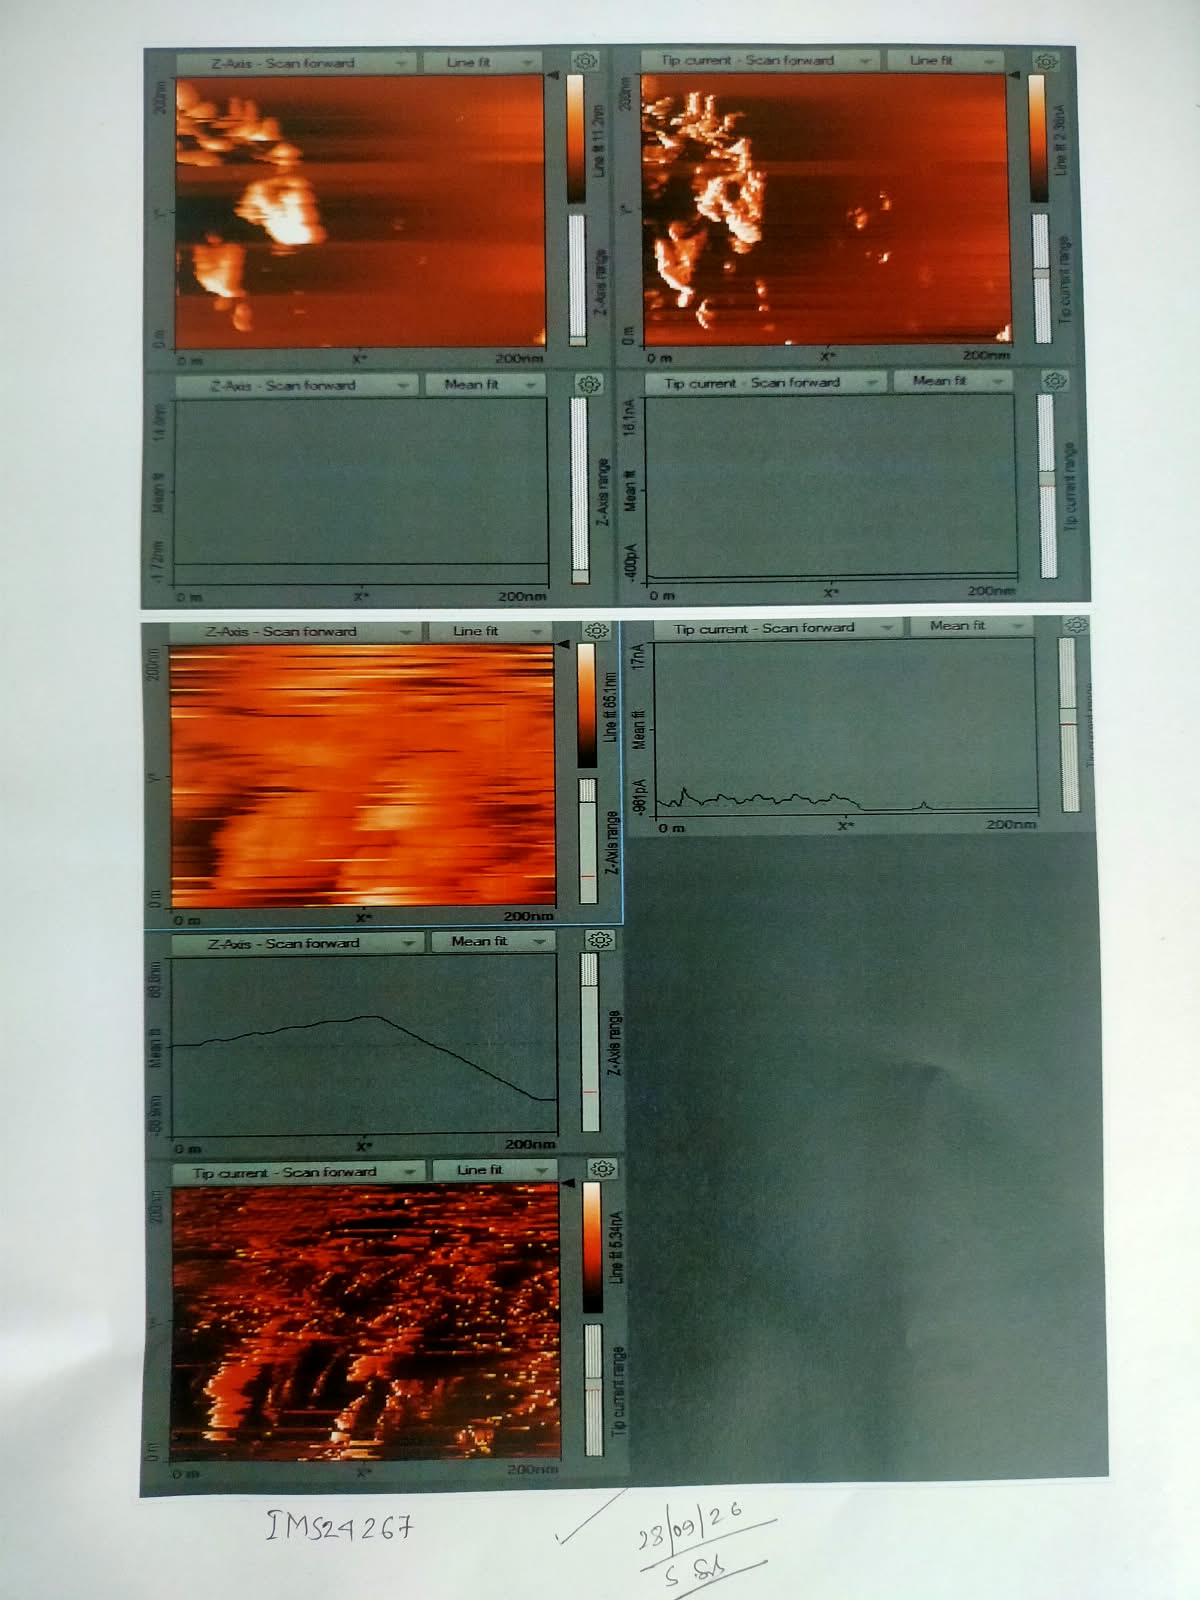
\includegraphics[width=0.9\textwidth]{signed-observation.jpeg}
    \caption{Signed lab observation sheet.}
    \label{fig:signed-obs}
\end{figure}

\end{document}
